\chapter{SYSTEM ANALYSIS AND DESIGN}
    \section{Functional Requirements}
    Functional requirements define the fundamental actions that system must perform. The functional requirements for the system are divided into three main categories: Reservation, Food, and Management. 
    \begin{enumerate}
        \item Reservation
        \begin{itemize}
            \item The system shall reservations.
            \item The system shall record the customer's information such as: their first name, last name, phone number.
            \item The system shall record the number of occupants.
            \item The system shall record the room number.
            \item The system shall display the room rate.
            \item The system shall generate a unique confirmation number for each reservation.
            \item The system shall automatically cancel reservations after 6 hours check-in time if the customer has not checked in.
            \item The system shall record the expected check-in date.
            \item The system shall record the expected checkout date.
            \item The system shall record the airport transfer booking (if any).
            \item The system shall check in customers.
            \item The system shall allow reservations to be modified some information.
            \item The system shall check out customers.
            \begin{itemize}
                \item The system shall display the amount owed by the customer.
                \item The system shall record that the room status is available.
                \item The system shall record the invoice.
            \end{itemize}
            \item The system shall record customer feedback.
        \end{itemize}
        \item Food
        \begin{itemize}
            \item The system shall track all meals purchased in the hotel.
            \item The system shall bill the current room if payment is not made at the time of service.
        \end{itemize}
        \item Management 
        \begin{itemize}
            \item The system shall display the hotel occupancy for a specified period (days).
            \item The system shall display projected occupancy for a period of time (days).
            \item The system shall display room revenue.
            \item The system shall display food revenue.
            \item The system shall display customer feedback.
            \item The system shall allow manager to create new user.
            \item The system shall allow for the addition of information, regarding rooms, rates, menu items, prices, reservations and user profile.
            \item The system shall allow for the modification of information, regarding rooms, rates, menu items, prices, reservations and user profile.
            \item The system shall allow for the deletion of information, regarding rooms, rates, menu items, prices, and user profile.
        \end{itemize}
    \end{enumerate}
    \section{Non-functional Requirements}
    \begin{enumerate}
        \item Performance
\newline Performance requirements define acceptable response time for system functionality.
        \item Security
        \newline Security is also a major factor that needs to be handled carefully on every web application that allows
the user to log in with accounts. The information provided by the users will be stored in a private database and the user’s password will be hashed before storing in order to protect it from being exposed. HMS also has a separate route for the administrators to access the admin dashboard and prevent unauthorized access from normal users. 
        \item Availability
\newline     HMS is expected to be available 24 hours a day and the users can access the website at any time. Users can access the website from anywhere in the world, however, for receptionists and managers, need to log in with their account (provided before) to access all the functionalities of the website.
        \item Maintainability
\newline        The hotel requirements are rapidly changing with the open economy and the system must be able to change rapidly. So to develop a new system in each change is not a possible task. So re-usability of components and maintainability of the system are very important.
    \end{enumerate}
    
    \section{Use-case Diagram}
    \subsection{Use-case diagram}
    \begin{figure}[H]
        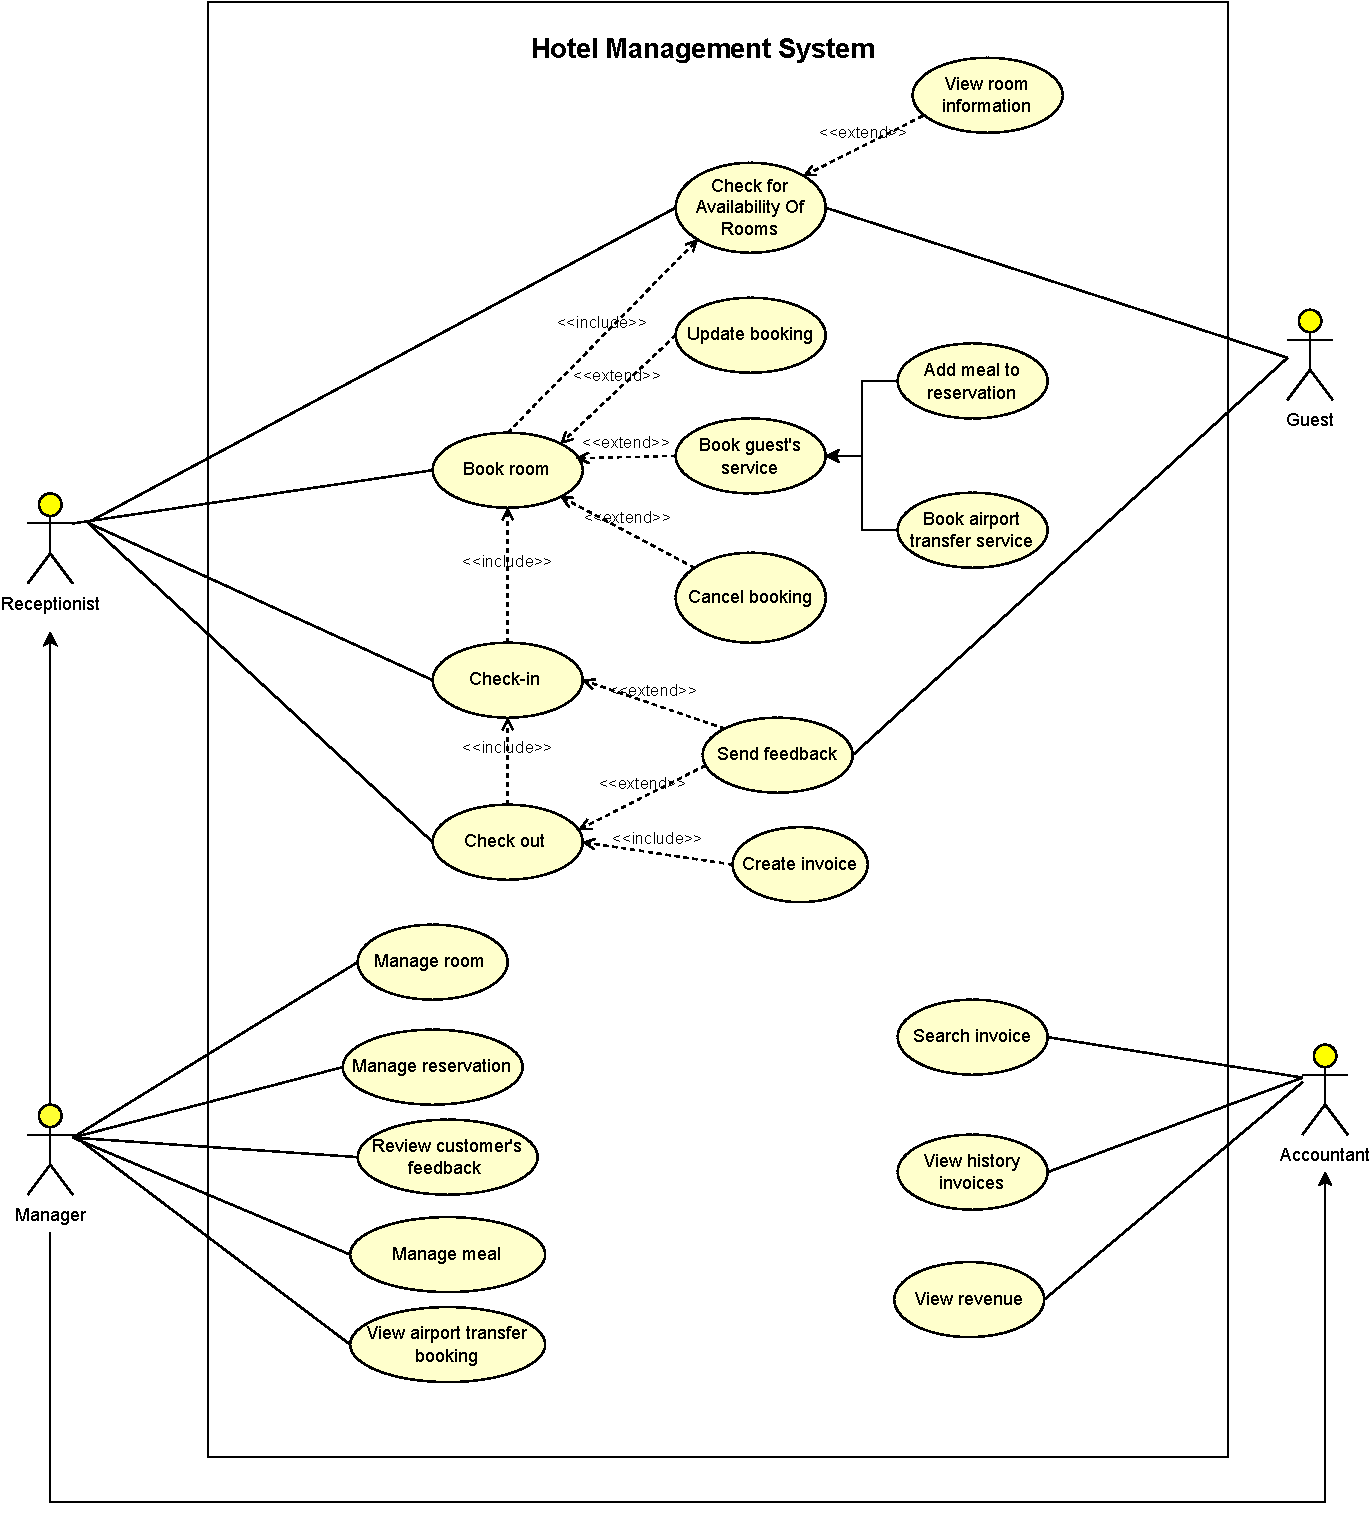
\includegraphics[width=\textwidth]{img/usecase-diagram.pdf}
        \caption{Use-case Diagram }
        \label{fig: Use-case Diagram }
    \end{figure}
    \subsection{Use-case description}
    There are 4 actors and 16 use-cases.
    
\begin{table}[htb]
\begin{tabular}{|>{\raggedright\arraybackslash}p{6cm}|>{\raggedright\arraybackslash}p{10cm}|}
\hline
\textbf{Actors}& \textbf{Description}\\
\hline
\multirow{2}{*}{Guest}& Check for available rooms \\
& Send feedback\\
\hline
\multirow{3}{*}{Receptionist}& Booking \\
& Cancel booking \\
& Update booking \\
& Check for available rooms \\
& View room information \\
& Check in \\
& Check out \\
& Book airport transfer service \\
& Book meals \\
& Send feedback \\
\hline
\multirow{2}{*}{Accountant}& Search invoice \\
& View history invoice\\
\hline
\multirow{3}{*}{Manager}& Manage room\\
& Manage reservation \\
& Manage menu items \\
& Review guest's feedback \\
& View guest's services\\
& All right of accountant and receptionist\\
\hline
\end{tabular}
\caption{List of actors of system}
\label{tab:actors}
\end{table}

%list of use-cases
%list of use-cases
\begin{table}
\begin{tabular}{|>{\raggedright\arraybackslash}p{1cm}|>{\raggedright\arraybackslash}p{3cm}|>{\raggedright\arraybackslash}p{8cm}|>{\raggedright\arraybackslash}p{3cm}|}
\hline
\textbf{ID}& \textbf{Use-Case}& \textbf{Description}& \textbf{Actor}\\
\hline
UC01& Login& Actor login to the system. Depending on the account type, there are different functions& Manager, Receptionist, Accountant \\
\hline
UC02& Check for available rooms &Actor enters the system to check whether the room is available or unavailable & Guest, Receptionist, Manager\\
\hline
UC03& Booking & Actor books rooms for guests and services such as vehicles and meals if guests need them.& Receptionist, Manager\\
\hline
UC04& Update booking&Actor edits reservation information for guests and services such as vehicle and meal & Receptionist, Manager\\
\hline
UC05& Cancel booking&Actor cancels booking information for guests and services. & Admin, Repository manager\\
\hline
UC06& View room information &Actor views room information (room price, room equipment, and room status) & Guest, Receptionist, Manager\\
\hline 
UC07& Book meals& Actor book meals for guests, including name, quantity, type, and additional notes. & Receptionist, Manager\\
\hline
UC08& Book airport transfer service& Actor book transfer service to take guests from the airport to the hotel. & Receptionist, Manager\\
\hline
UC09& Check-in & Actor checks the guest's check-in time. & Receptionist, Manager\\
\hline
UC10& Check out& Actor checks the time a guest leaves a hotel room. & Receptionist, Manager\\
\hline
UC11& Send feedback& Actor evaluates the hotel's service quality and the staff's service attitude. & Receptionist, Guest \\
\hline
UC12& Find invoice& Actor search the list of issued invoices& Accountant, Manager\\
\hline 
UC13& View invoice history& Actor views the history of invoices and views their details& Accountant, Manager\\
\hline 
UC14& Manage room& Actor manages room status, facilities, images and prices of the room& Manager\\
\hline 
UC15& Manage reservation & Actor manages check-in time, check-out of rooms that guests have reserved, and services such as vehicles and meals & Manager\\
\hline 
UC16& Manage menu item& Actor manages the list of meals to be served to guests (editing, adding and deleting meal) & Manager\\
\hline 
UC17& Review guest's feedback& Actor views guest's feedback after they use hotels and other services.
 & Manager\\
\hline 
UC18& View all airport transfer services& Actor looks at all the vehicles that the hotel offers to guests. & Manager\\
\hline 
\end{tabular}
\caption{List of Use-Cases of system}
\label{tab:use-cases}
\end{table}


% specification
% mỗi bảng đặc tả bao gồm tên Use-case, tác nhân chính và phụ, mô tả, hoạt động/ tác nhân kích hoạt, mối quan hệ Use-case (Include/Extend), luồng hoạt động chính, luồng hoạt động thay thế
% UC1
\begin{table}
\begin{tabular}{|>{\raggedright\arraybackslash}p{5cm}|>{\raggedright\arraybackslash}p{10cm}|}
\hline
ID& UC01 \\
\hline
Use-Case Name& Login \\
\hline
Actors& Manager, Receptionist, Accountant\\
\hline
Brief Description& Actor login to the system. Depending on
the account type, there are different functions and perform different operations. \\
\hline
Trigger& Actor wants to log in to the website \\
\hline
Preconditions & Actor already has an account on the system \\
\hline
Postconditions& Actor successfully logs into the system and performs its functions \\
\hline
Flow& 1.1 Manager, Accountant and receptionist log in to the website homepage and enter the link to access with permission: localhost:8080/@role.\\& 1.2 The system will take the actor to the login page
\\ &1.3 Actor enters username and password. Then actor clicks login.
\\
\hline
Alternatives& \\
\hline
\end{tabular}

\caption{UC01 Login}
\label{tab:UC01}
\end{table}
% UC2
\begin{table}
\begin{tabular}{|>{\raggedright\arraybackslash}p{5cm}|>{\raggedright\arraybackslash}p{10cm}|}
\hline
ID& UC02 \\
\hline
Use-Case Name&  Check for availability Of Rooms\\
\hline
Actors& Receptionist, Guest, Manager\\
\hline
Brief Description& The users check rooms ready for use based on their specific requirement \\
\hline
Trigger& Actor is on the system's home page\\
\hline
Preconditions& Actor successfully accessed the website.\\
\hline
Postconditions& Actor successfully view the room's details  \\
\hline
Flow& 2.1 Guest, Receptionist, and Manager access the home page\\&2.2 Actor fills in all fields such as the time they will check in, check out, and the number of people who will rent the room(including adults and children)\\ &2.3 The system displays available room information to the actor.
\\
\hline
Alternatives& \\
\hline
\end{tabular}

\caption{UC02  Check for availability Of Rooms}
\label{tab:UC02}
\end{table}
% UC3
\begin{table}
\begin{tabular}{|>{\raggedright\arraybackslash}p{5cm}|>{\raggedright\arraybackslash}p{10cm}|}
\hline
ID& UC03 \\
\hline
Use-Case Name& Booking\\
\hline
Actors& Receptionist, Manager\\
\hline
Brief Description& Actor receives advance reservations from guest\\
\hline
Trigger& Actor clicks “Add Booking room” on the toolbar in the "Front desk".\\
\hline
Preconditions & Actor successfully logs into the system and the hotel has available rooms \\
\hline
Postconditions& Room booked successfully\\
\hline
Flow& 3.1 Actor clicks on the "Front desk" on the toolbar \\ &3.2 The system displays room information for actor \\& 3.3 Actor selects an available room and fills in guest information.\\& 3.4 Actor adds additional services if customers need them, such as meal and airport transfer services\\& Actor confirms the room has been booked.
\\
\hline
Alternatives& \\
\hline
\end{tabular}

\caption{UC03 Booking}
\label{tab:UC03}
\end{table}
% UC04
\begin{table}
\begin{tabular}{|>{\raggedright\arraybackslash}p{5cm}|>{\raggedright\arraybackslash}p{10cm}|}
\hline
ID& UC04 \\
\hline
Use-Case Name& Update booking\\
\hline
Actors& Receptionist, Manager\\
\hline
Brief Description& Actor updates booking information for guests, changes service details\\
\hline
Trigger& Actor clicks on the "Reservation" on the toolbar and then select the edit item in the menu of a reservation you want to edit.\\
\hline
Preconditions & Actor successfully logged into the system and the hotel had a room booked.\\
\hline
Postconditions& Updated successfully\\
\hline
Flow& 4.1 Actor clicks on the "Reservation" on the toolbar \\ &4.2 The system displays information about the room booked\\& 4.3  Actor selects the edit item in the menu of a reservation you want to edit
\\& 4.4 The system displays information about the room booked, the guest, and services that the guest has booked for actor \\& 4.5 Actor edits the information they want to change in the reservation.\\
\hline
Alternatives& \\
\hline
\end{tabular}

\caption{UC04 Update booking}
\label{tab:UC04}
\end{table}
% UC05
\begin{table}
\begin{tabular}{|>{\raggedright\arraybackslash}p{5cm}|>{\raggedright\arraybackslash}p{10cm}|}
\hline
ID& UC05 \\
\hline
Use-Case Name& Cancel booking\\
\hline
Actors& Receptionist, Manager\\
\hline
Brief Description& Actor cancels the guest's reservation\\
\hline
Trigger& Actor clicks on the "Reservation" on the toolbar and then actor select the edit item in the menu of a reservation you want to cancel.\\
\hline
Preconditions & Actor successfully logs into the system and the hotel had a room booked\\
\hline
Postconditions& Cancelled successfully\\
\hline
Flow& 5.1 The receptionist clicks on the "Reservation" on the toolbar \\ &5.2 The system displays information about the room booked, the guest, and services that the guest has booked for Actor \\& 5.3 Actor Actor selects "Edit" and changes the room's status to canceled and will cancel the booking from the guest.
\\
\hline
Alternatives& \\
\hline
\end{tabular}

\caption{UC05 Cancel booking}
\label{tab:UC05}
\end{table}

% UC06
\begin{table}
\begin{tabular}{|>{\raggedright\arraybackslash}p{5cm}|>{\raggedright\arraybackslash}p{10cm}|}
\hline
ID& UC06 \\
\hline
Use-Case Name& View room information\\
\hline
Actors& Receptionist, Manager, Guest\\
\hline
Brief Description& Actor views detail information about the room (images, facilities, price, etc.)\\
\hline
Trigger& Actor views detailed information about the room on the home page\\
\hline
Preconditions & Actor successfully logs into the system and the system has room to show \\
\hline
Postconditions & View room information successfully\\
\hline
Flow& 6.1 Actor goes to the home page of the website\\ &6.2 The system displays room information for Actor.
\\
\hline
Alternatives& \\
\hline
\end{tabular}

\caption{UC06 View room information}
\label{tab:UC05}
\end{table}

% UC07
\begin{table}
\begin{tabular}{|>{\raggedright\arraybackslash}p{5cm}|>{\raggedright\arraybackslash}p{10cm}|}
\hline
ID& UC07 \\
\hline
Use-Case Name& Book Meals\\
\hline
Actors& Manager, Receptionist\\
\hline
Brief Description& Actor booking meals for guests \\
\hline
Trigger& While booking a room for a guest, the "Meal" section will appear, where the Actor will add food according to the guest's request.\\
\hline
Preconditions & Actor successfully logs into the system and meals available\\
\hline
Postconditions& Book meals successfully\\
\hline
Flow& 7.1 Actor clicks on the "Front desk" and then clicks on the "Add booking room"\\ & 7.2 The system displays information for booking room and then the system displays information board for actor to book meals for guests after actor have filled in all guest information and selected a room to book\\& 7.3 Actor enters the information of the guest who booked the meal and chooses the meal that the guest has booked.
\\
\hline
Alternatives& 7.4 Actor clicks on the "reservation" and then clicks on the "add meals"\\ &7.5 The system displays an information board for actor to book meals for guests. \\& Actor chooses the meal that the guest has booked.\\
\hline
\end{tabular}

\caption{UC07 Book meals}
\label{tab:UC07}
\end{table}

% UC08
\begin{table}
\begin{tabular}{|>{\raggedright\arraybackslash}p{5cm}|>{\raggedright\arraybackslash}p{10cm}|}
\hline
ID& UC08 \\
\hline
Use-Case Name& Book airport transfer service\\
\hline
Actors& Manager, Receptionist\\
\hline
Brief Description& Actor booking airport transfer service for guests \\
\hline
Trigger& While booking a room for a guest, the "Vehicle" section will appear, where the actor will choose the vehicle and place to pick up to guest's request.\\
\hline
Preconditions & Actor successfully logs into the system and vehicle available \\
\hline
Postconditions & Book airport transfer service successfully \\
\hline
Flow& 8.1. Actor clicks on the "Front desk" and then clicks on the "Add booking room"\\ & 8.2 The system displays information for booking room and then the system displays information board for actor to book airport transfer service for guests after actor have filled in all guest information and selected a room to book.\\& 8.3 Actor enters the information of the guest who booked the airport transfer service and chooses the vehicle and place to pick up that the guest has booked.
\\
\hline
Alternatives& \\
\hline
\end{tabular}

\caption{UC08 Book airport transfer service}
\label{tab:UC08}
\end{table}

% UC09
\begin{table}
\begin{tabular}{|>{\raggedright\arraybackslash}p{5cm}|>{\raggedright\arraybackslash}p{10cm}|}
\hline
ID& UC09 \\
\hline
Use-Case Name& Check-in\\
\hline
Actors& Receptionist, Manager\\
\hline
Brief Description& Actor confirms that the room has been booked by the guest (guest check-in time)\\
\hline
Trigger& Actor clicks “Reservation” on the toolbar and edits the room's status.\\
\hline
Preconditions & Actor successfully logs into the system and previously booked room successfully or the hotel has available rooms for guests to book\\
\hline
Postconditions & Confirm the guest has successfully checked in\\
\hline
Flow& 9.1. Actor clicks on the "Reservation" on the toolbar \\ &9.2  The system displays information about the room booked, the guest, and services that the guest has booked for Actor \\& 9.3 Actor edits the room's status - Confirm the room is occupied("check-in").
\\
\hline
Alternatives& \\
\hline
\end{tabular}

\caption{UC09 Check-in}
\label{tab:UC09}
\end{table}
% UC010
\begin{table}
\begin{tabular}{|>{\raggedright\arraybackslash}p{5cm}|>{\raggedright\arraybackslash}p{10cm}|}
\hline
ID& UC010 \\
\hline
Use-Case Name& Check out\\
\hline
Actors& Receptionist, Manager\\
\hline
Brief Description& Actor confirms that the guest has left the room (guest check out time)\\
\hline
Trigger& Actor clicks “Room” on the toolbar and edits the room's status.\\

\hline
Preconditions & Actor successfully logged into the system and checked in successfully\\
\hline
Postconditions& Confirm the guest has successfully checked out\\
\hline
Flow& 10.1. Actor clicks on the "Reservation" on the toolbar \\ & 10.2The system displays information about the room booked, the guest, and services that the guest has booked for Actor \\& 10.3 Actor edits the room's status -Confirm the guest has left the room("checkout")
\\
\hline
Alternatives& \\
\hline
\end{tabular}

\caption{UC010 Check out}
\label{tab:UC010}
\end{table}

% UC011
\begin{table}
\begin{tabular}{|>{\raggedright\arraybackslash}p{5cm}|>{\raggedright\arraybackslash}p{10cm}|}
\hline
ID& UC011 \\
\hline
Use-Case Name& Send feedback\\
\hline
Actors&Guest, Receptionist\\
\hline
Brief Description& Actor send reviews about hotel quality, service, and staff attitude to the hotel\\
\hline
Trigger& Actor clicks on "feedback" on the toolbar on the home page.\\
\hline
Preconditions & Actor successfully logs into the system, reservation ID and phone must be present in the system data \\
\hline
Postconditions &  Confirm the room has been check out by the guest\\
\hline
Flow& 11.1. Actor clicks on the "feedback" \\ &11.2 The system displays a feedback board for actor and gives detailed feedback information for actor evaluate.\\ &11.3 Actor enters reservation ID and phone then writes problems when using the hotel.
\\
\hline
Alternatives& 11.4 The receptionist goes to his or her own work page and selects "Send feedback" on the toolbar.\\& 11.5 The system displays a response panel to the agent and provides detailed feedback.\\&  The receptionist enters reservation ID and phone then writes problems.\\
\hline
\end{tabular}

\caption{UC011 Send feedback}
\label{tab:UC011}
\end{table}

%UC12
\begin{table}
\begin{tabular}{|>{\raggedright\arraybackslash}p{5cm}|>{\raggedright\arraybackslash}p{10cm}|}
\hline
ID& UC012 \\
\hline
Use-Case Name& Find invoice\\
\hline
Actors& Accountant, Manager\\
\hline
Brief Description& Accountant, Manager look for certain invoice \\
\hline
Trigger&  Accountant, Manager click “Find invoice” in the "Invoice". \\
\hline
Preconditions & Actor successfully logs into the system \\
\hline
Postconditions& Guest or Receptionist sent feedback successfully\\
\hline
Flow& 12.1.   Accountant, Manager click “Invoice” on the toolbar \\ & 12.2 The system displays a list of invoices \\ & 12.3 Accountant, Manager click “Search now” and enter the invoice code  \\& 12.4 The system displays detailed information of the invoice.
\\
\hline
Alternatives& \\
\hline
\end{tabular}

\caption{UC012 Find invoice }
\label{tab:UC012}
\end{table}

%UC13
\begin{table}
\begin{tabular}{|>{\raggedright\arraybackslash}p{5cm}|>{\raggedright\arraybackslash}p{10cm}|}
\hline
ID& UC013 \\
\hline
Use-Case Name& View invoice history\\
\hline
Actors& Accountant, Manager\\
\hline
Brief Description& Actor reviews the history of invoices\\
\hline
Trigger&  Accountant, Manager click “Invoice” on the toolbar \\
\hline
Preconditions &  Actor successfully logs into the system\\
\hline
Postconditions& Actor successfully viewed existing invoices.\\
\hline
Flow& 13.1.   Accountant, Manager click “Invoice” on the toolbar \\ & 13.2 The system displays a list of invoices \\
\\
\hline
Alternatives& \\
\hline
\end{tabular}

\caption{UC013 View invoice history}
\label{tab:UC013}
\end{table}

% UC014
\begin{table}
\begin{tabular}{|>{\raggedright\arraybackslash}p{5cm}|>{\raggedright\arraybackslash}p{10cm}|}
\hline
ID& UC014 \\
\hline
Use-Case Name& Manage Room\\
\hline
Actors& Manager\\
\hline
Brief Description&The manager uses it to manage room in the hotels\\
\hline
Trigger& The manager clicks on "Room" on the toolbar\\
\hline
Preconditions &  Actor successfully logs into the system\\
\hline
Postconditions& \\
\hline
Flow&  14.1 The manager clicks on the "Room" on the sidebar\\& 14.2 The system displays a list of rooms for the actor \\ & 14.3 The manager chooses the function he wants to perform: \\ & 14.3.1 If the manager chooses to add or edit room information. After entering or adjusting all information about the room that needs to be edited (or added), the manager clicks on "Add" or "Save", and the room information in the hotel is automatically added to the database table.\\ & 14.3.2 If the manager chooses to delete, the system requires the manager to enter the exact room code to be deleted, and then confirm, that information about that room will be deleted from the system's database table.
\\
\hline
Alternatives& \\
\hline
\end{tabular}

\caption{UC04 Manage Room}
\label{tab:UC014}
\end{table}
% UC015
\begin{table}
\begin{tabular}{|>{\raggedright\arraybackslash}p{5cm}|>{\raggedright\arraybackslash}p{10cm}|}
\hline
ID& UC015 \\
\hline
Use-Case Name& Manage Reservation\\
\hline
Actors& Manager\\
\hline
Brief Description&The manager uses it to manage room reservations in the hotels\\
\hline
Trigger&  The manager clicks on "Reservation" on the toolbar.\\
\hline
Preconditions & Actor successfully logs into the system\\
\hline
Postconditions& \\
\hline
Flow& 15.1 The manager clicks on the "Reservation"\\ & 15.2 The system displays a list of rooms for the actor \\ & 15.3 The manager chooses the function he wants to perform: \\ & 15.3.1 If the manager chooses to edit reservation information. After adjusting information about the reservation that needs to be adjusted, the manager clicks "Save", and the reservation information in the hotel is automatically added to the database table.\\& 15.3.2 If the manager chooses to add meals. They will select meal and quantity then press "Save". This is done when guests need food.
\\
\hline
Alternatives& \\
\hline
\end{tabular}

\caption{UC015 Manage Reservation}
\label{tab:UC015}
\end{table}

% UC016
\begin{table}
\begin{tabular}{|>{\raggedright\arraybackslash}p{5cm}|>{\raggedright\arraybackslash}p{10cm}|}
\hline
ID& UC016 \\
\hline
Use-Case Name& Manage menu item\\
\hline
Actors& Manager\\
\hline
Brief Description&The manager uses it to manage meal service in the hotels\\
\hline
Trigger&  The manager clicks on "Meal" on the toolbar.\\
\hline
Preconditions & Actor successfully logs into the system\\
\hline
Postconditions& \\
\hline
Flow& 16.1 The manager clicks on "Meal" on the sidebar\\ & 16.2 The manager chooses the function he wants to perform: \\ & 16.2.1 If the manager chooses to add or edit meal information. After entering or adjusting all information about the meal that needs to be adjusted (or added), the manager clicks on "Add" or "Save", and the meal information in the hotel is automatically added to the database table.\\ & 16.2.2 If the manager chooses to delete, the system requires the manager to enter the exact meal code to be deleted, and then confirm, that information about that meal will be deleted from the system's database table.
\\
\hline
Alternatives& \\
\hline
\end{tabular}

\caption{UC016 Manage menu item}
\label{tab:UC016}
\end{table}

% UC017
\begin{table}
\begin{tabular}{|>{\raggedright\arraybackslash}p{5cm}|>{\raggedright\arraybackslash}p{10cm}|}
\hline
ID& UC017 \\
\hline
Use-Case Name&  Review guest's feedback\\
\hline
Actors& Manager\\
\hline
Brief Description& Manager views feedback that guests give after using the hotel\\
\hline
Trigger& The manager clicks on the "feedback" on the toolbar\\
\hline
Preconditions & Actor successfully logs into the system and guest have sent feedback\\
\hline
Postconditions& Actor successfully view feedback from guests or receptionists\\
\hline
Flow& 17.1. The manager clicks on "feedback" on the toolbar \\ & 17.2 The system displays a list of feedback from guests.
\\
\hline
Alternatives& \\
\hline
\end{tabular}

\caption{UC017 Review guest's feedback}
\label{tab:UC017}
\end{table}

% UC018
\begin{table}
\begin{tabular}{|>{\raggedright\arraybackslash}p{5cm}|>{\raggedright\arraybackslash}p{10cm}|}
\hline
ID& UC018 \\
\hline
Use-Case Name&  View all airport transfer services\\
\hline
Actors& Manager\\
\hline
Brief Description& Manager views all the vehicles guests using the airport transfer services\\
\hline
Trigger& Manager clicks on the "Services" on the toolbar\\
\hline
Preconditions & Actor successfully logs into the system\\
\hline
Postconditions& Actor successfully view all airport transfer services \\
\hline
Flow& 18.1. The manager clicks on "Services" on the toolbar \\ & 18.2 The system displays a list of services and includes information about pick-up location and vehicle information, etc
\\
\hline
Alternatives& \\
\hline
\end{tabular}

\caption{UC018 View all airport transfer services}
\label{tab:UC017}
\end{table}


\clearpage
\section{Data Flow Diagram}
\subsection{DFD Context}
\begin{figure}[H]
    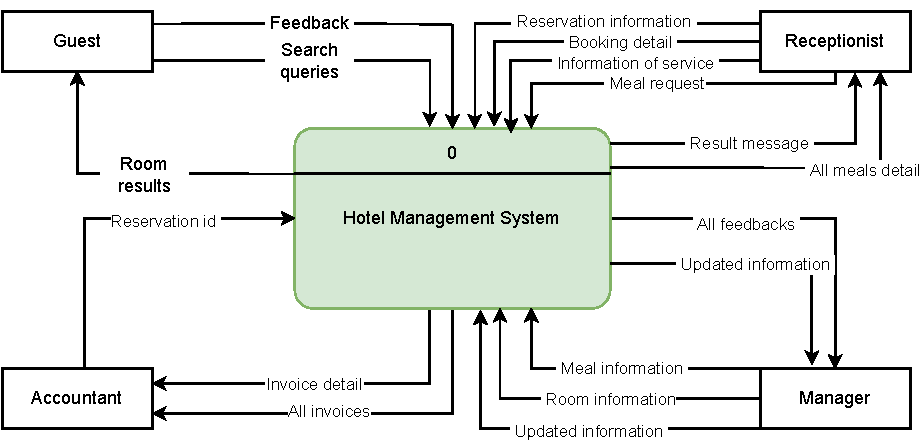
\includegraphics[width=1\linewidth]{img/dfd-context.pdf}
    \caption{DFD Context}
    \label{fig:DFD Context}
\end{figure}
\subsection{DFD Level-0}
* Overview \\
The below Data Flow Diagram (DFD) represents a Level-0 diagram for a Hotel Management System (HMS), focusing on several key processes and their interactions with external entities and data stores. The diagram includes the following components:
\begin{enumerate}
    \item Guest Interactions:
    \begin{itemize}
        \item Check for Available Rooms: The users initiate a room search query, and the system returns room results.
        \item Send Feedback: Guests can provide feedback, which is stored in the HMS's feedback data store.
    \end{itemize}
    \item Room and Reservation Management:
    \begin{itemize}
        \item Manage Room: This process involves updating room information based on guest check-ins, check-outs, and reservations.
        \item Book Room: Guests can book rooms, and the system records the booking information in the reservation data store.
        \item Check-In and Check-Out Processes: These are represented as individual processes, handling reservation information and updating the system accordingly.
    \end{itemize}
    \item Feedback:
    \begin{itemize}
        \item Review Guest Feedback: The manager can review feedback from guests stored in the feedback data store, facilitating improvements in service quality.
    \end{itemize}
    \item Accounting:
    \begin{itemize}
        \item Search Invoice: The accountant can search for invoices based on reservation IDs, and view invoice history, with all invoices stored in a dedicated invoice data store.
    \end{itemize}
    \item Meal and Transport Services:
    \begin{itemize}
        \item Manage Menu Item: This process involves updating meal information in the meal data store.
        \item Book Meals: Guests can book meals, and the system records meal details.
        \item Book Airport Transfer Service: Guests can book transport services, with booking information stored in a transport data store.
    \end{itemize}
\end{enumerate}
The diagram shows various data stores like Room, Feedback, Reservation, Invoice, Meal, Guest, and Transport, each storing relevant information for their respective processes. Entities like Guests, Managers, Receptionists, and Accountants interact with the system, providing inputs like queries, and information, and receiving outputs like room results and invoice details. This DFD provides a high-level overview of the core processes and data interactions within a Hotel Management System.
\begin{figure}[H]
    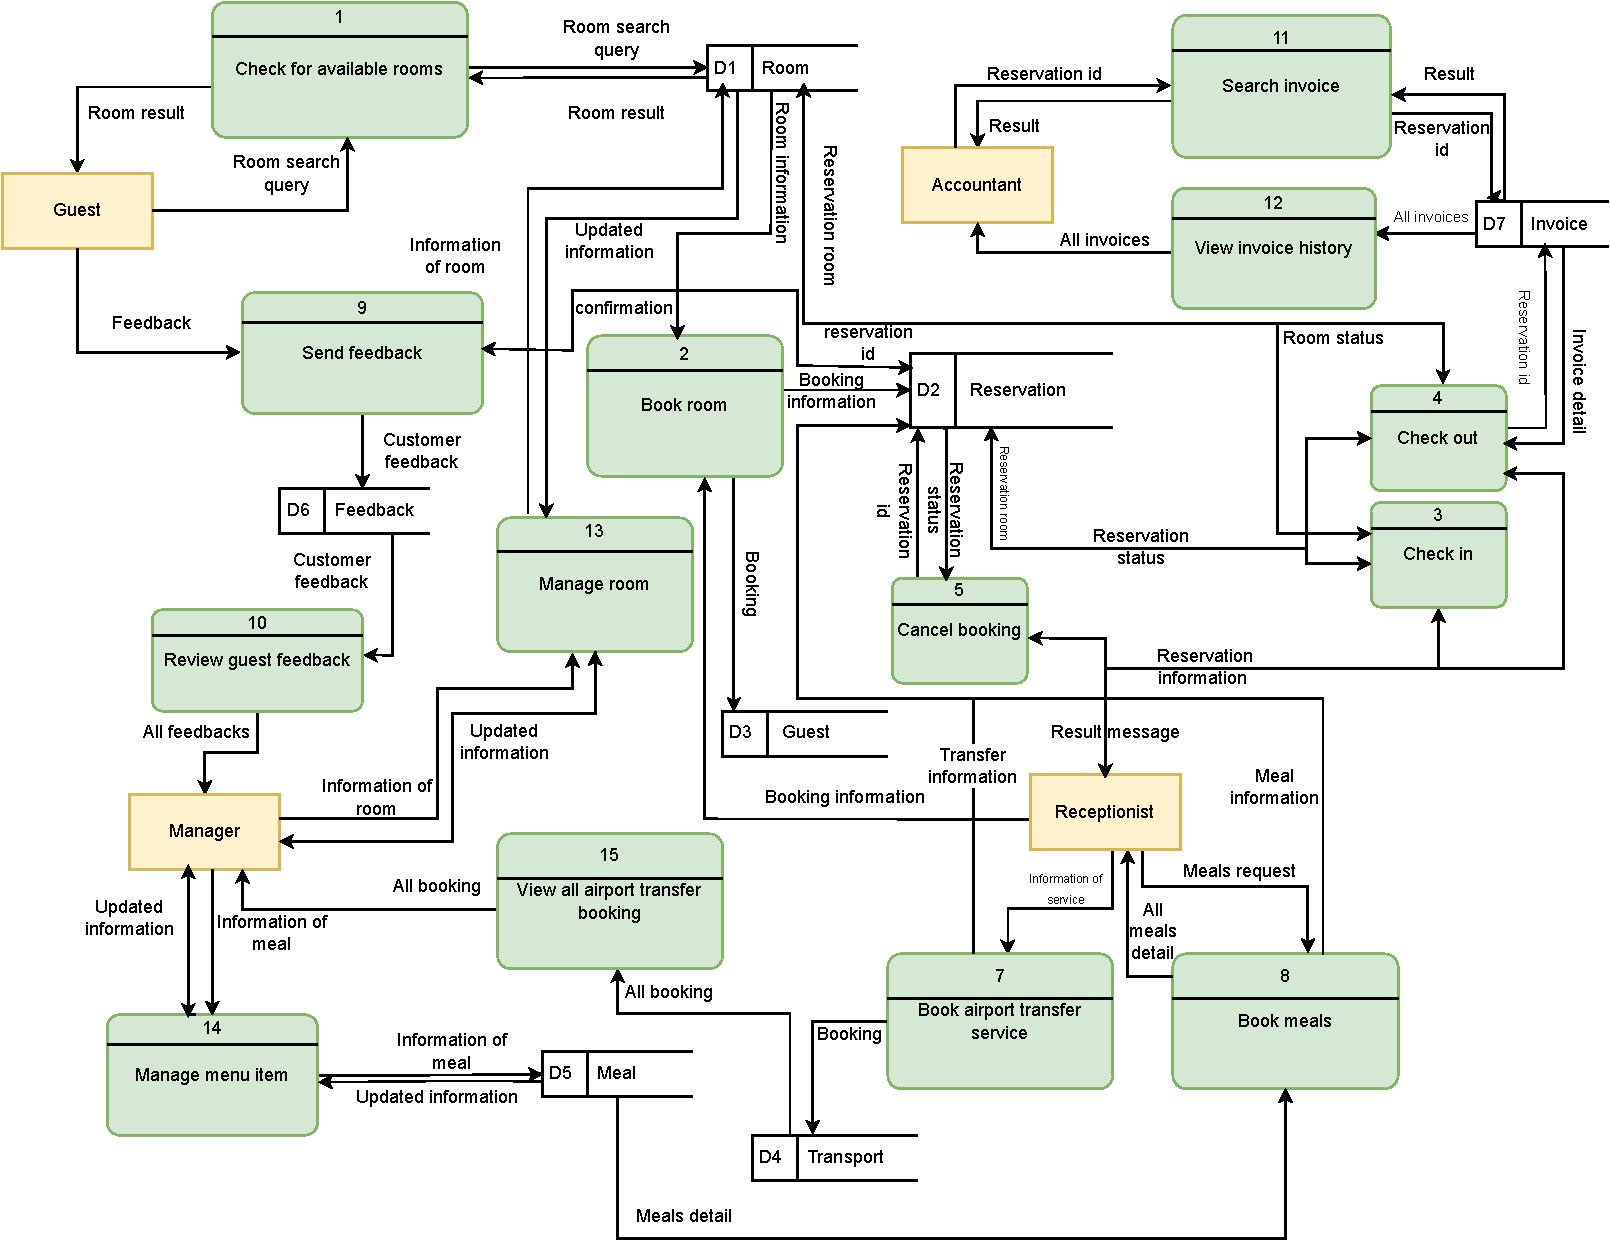
\includegraphics[width=1\linewidth]{img/dfd-0.drawio.pdf}
    \caption{DFD Level-0}
    \label{fig:DFD Level-0}
\end{figure}
* DFD Fragment
\begin{figure}[H]
    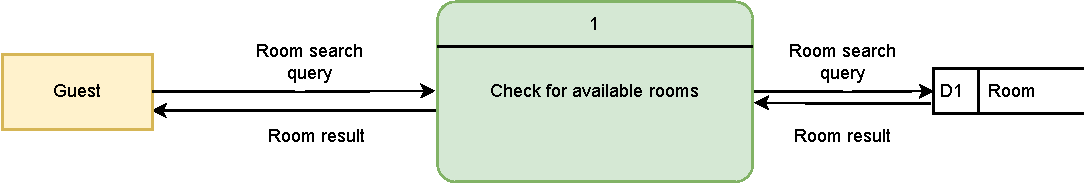
\includegraphics[width=1\linewidth]{img/dfd1.pdf}
    \caption{DFD Fragment of UC02}
    \label{fig:DFD Fragment of UC02}
\end{figure}
\begin{figure}[H]
    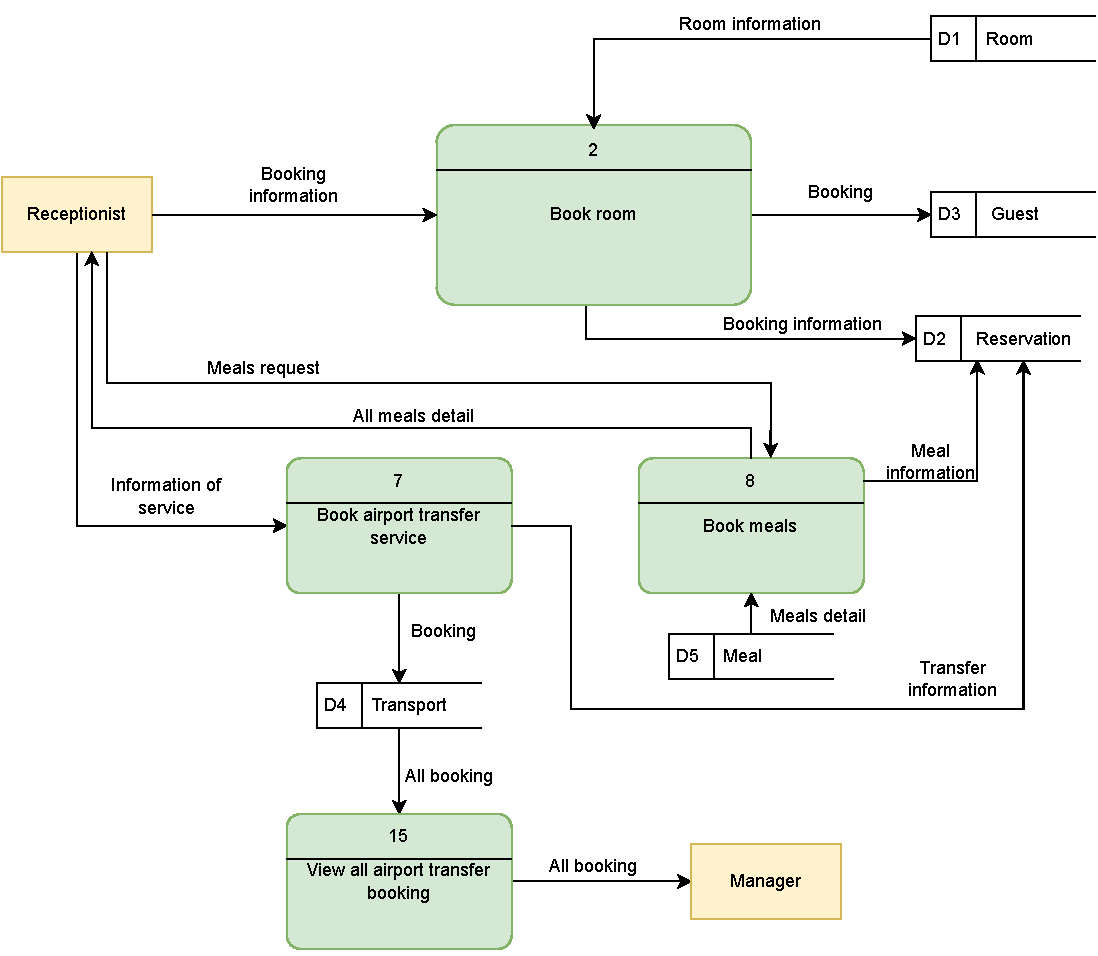
\includegraphics[width=1\linewidth]{img/dfd2.pdf}
    \caption{DFD Fragment of UC03,UC07,UC08}
    \label{fig:DFD Fragment of UC03,UC07,UC08}
\end{figure}
\begin{figure}[H]
    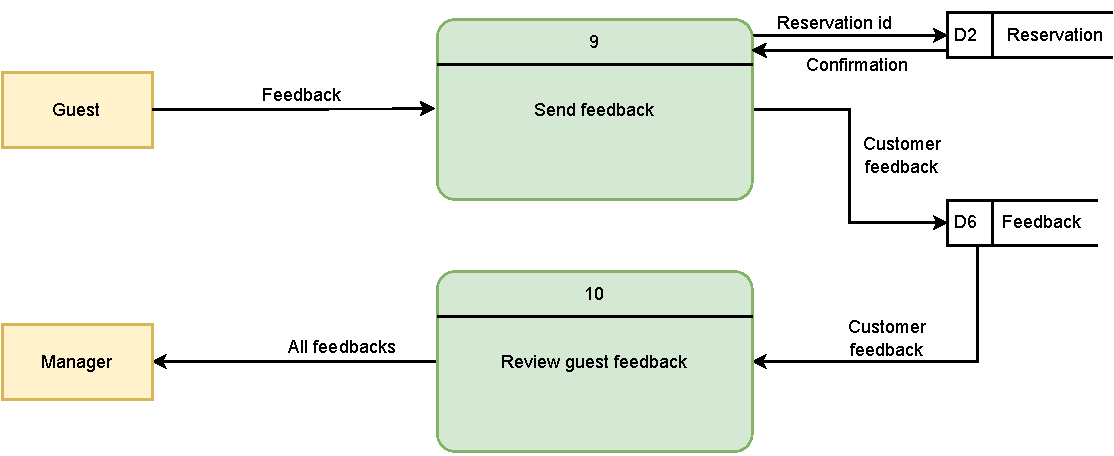
\includegraphics[width=1\linewidth]{img/dfd3.pdf}
    \caption{DFD Fragment of UC11,UC17}
    \label{fig:DFD Fragment of UC11,UC17}
\end{figure}
\begin{figure}[H]
    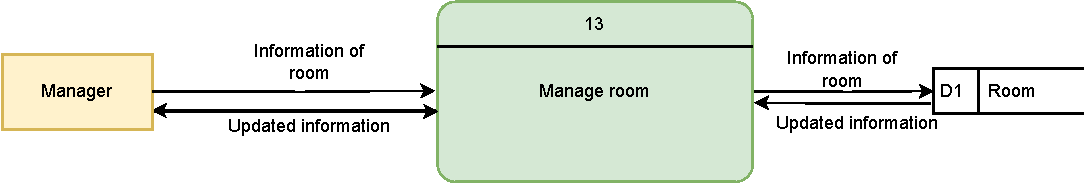
\includegraphics[width=1\linewidth]{img/dfd4.pdf}
    \caption{DFD Fragment of UC14}
    \label{fig:DFD Fragment of UC14}
\end{figure}
\begin{figure}[H]
    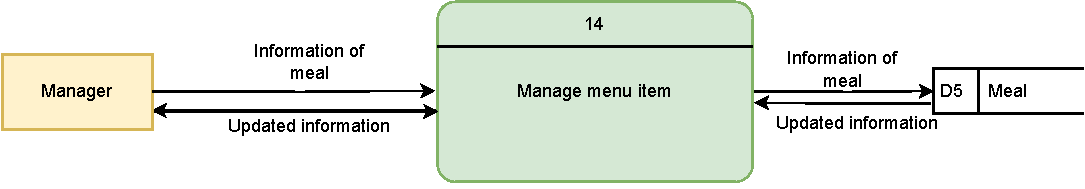
\includegraphics[width=1\linewidth]{img/dfd5.pdf}
    \caption{DFD Fragment of UC16}
    \label{fig:DFD Fragment of UC16}
\end{figure}
\begin{figure}[H]
    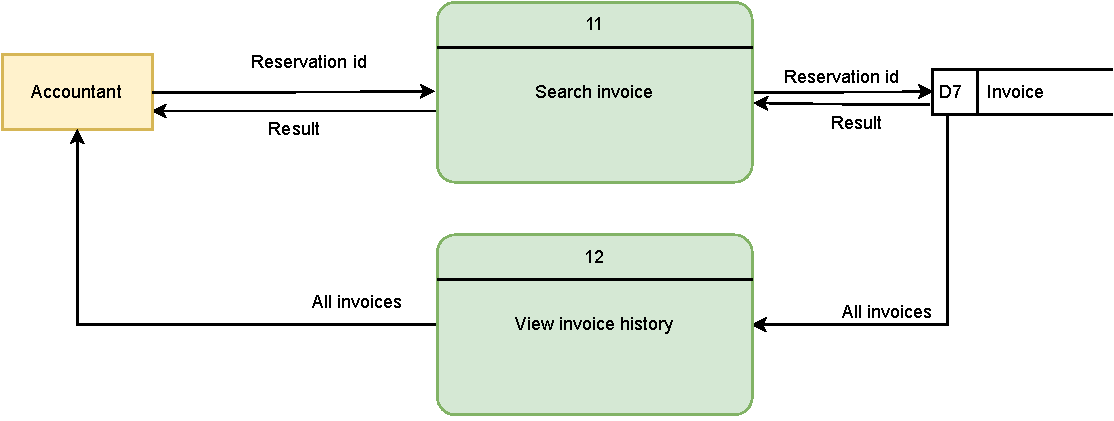
\includegraphics[width=1\linewidth]{img/dfd6.pdf}
    \caption{DFD Fragment of UC12,UC13}
    \label{fig:DFD Fragment of UC12,UC13}
\end{figure}
\begin{figure}[H]
    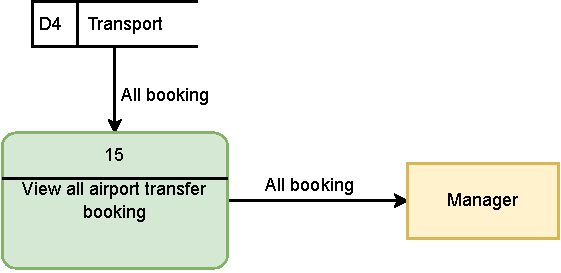
\includegraphics[width=1\linewidth]{img/dfd7.pdf}
    \caption{DFD Fragment of UC18}
    \label{fig:DFD Fragment of UC18}
\end{figure}
\begin{figure}[H]
    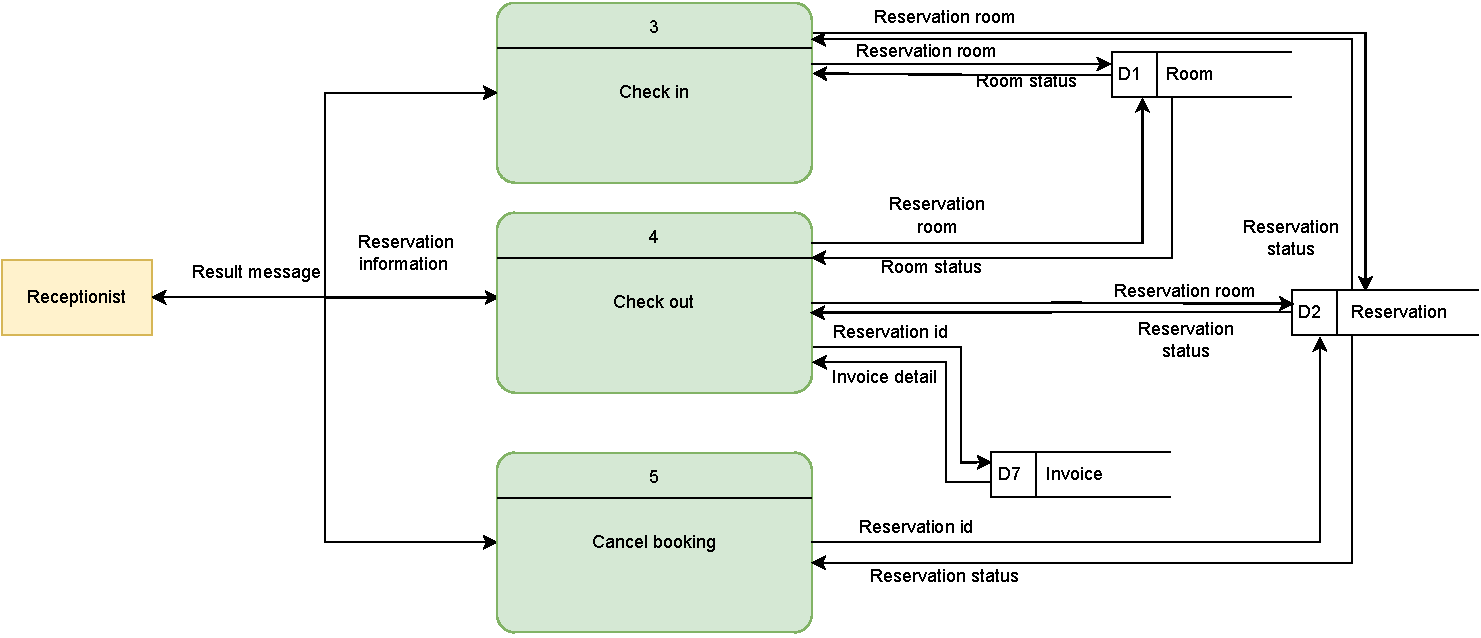
\includegraphics[width=1\linewidth]{img/dfd8.pdf}
    \caption{DFD Fragment of UC05,UC09,UC10}
    \label{fig:DFD Fragment of UC05,UC09,UC10}
\end{figure}
\begin{figure}[H]
    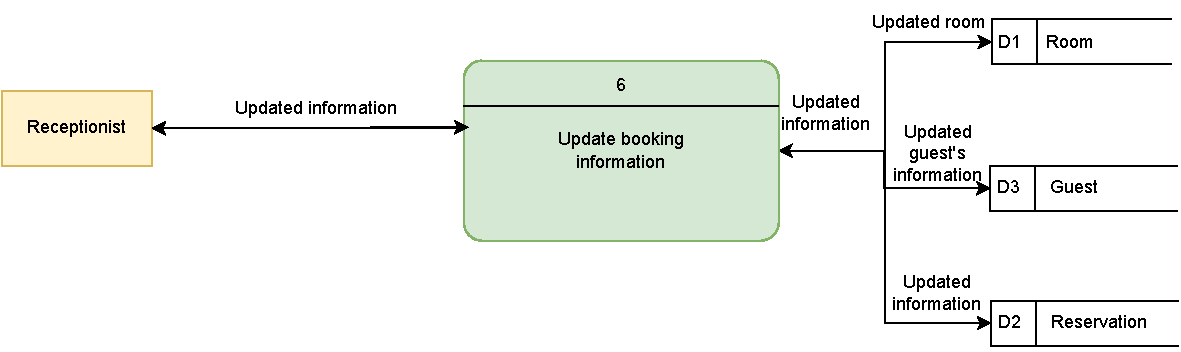
\includegraphics[width=1\linewidth]{img/dfd9.pdf}
    \caption{DFD Fragment of UC04}
    \label{fig:DFD Fragment of UC04}
\end{figure}

\section{Entity-Relationship Diagram}
\begin{figure}[H]
        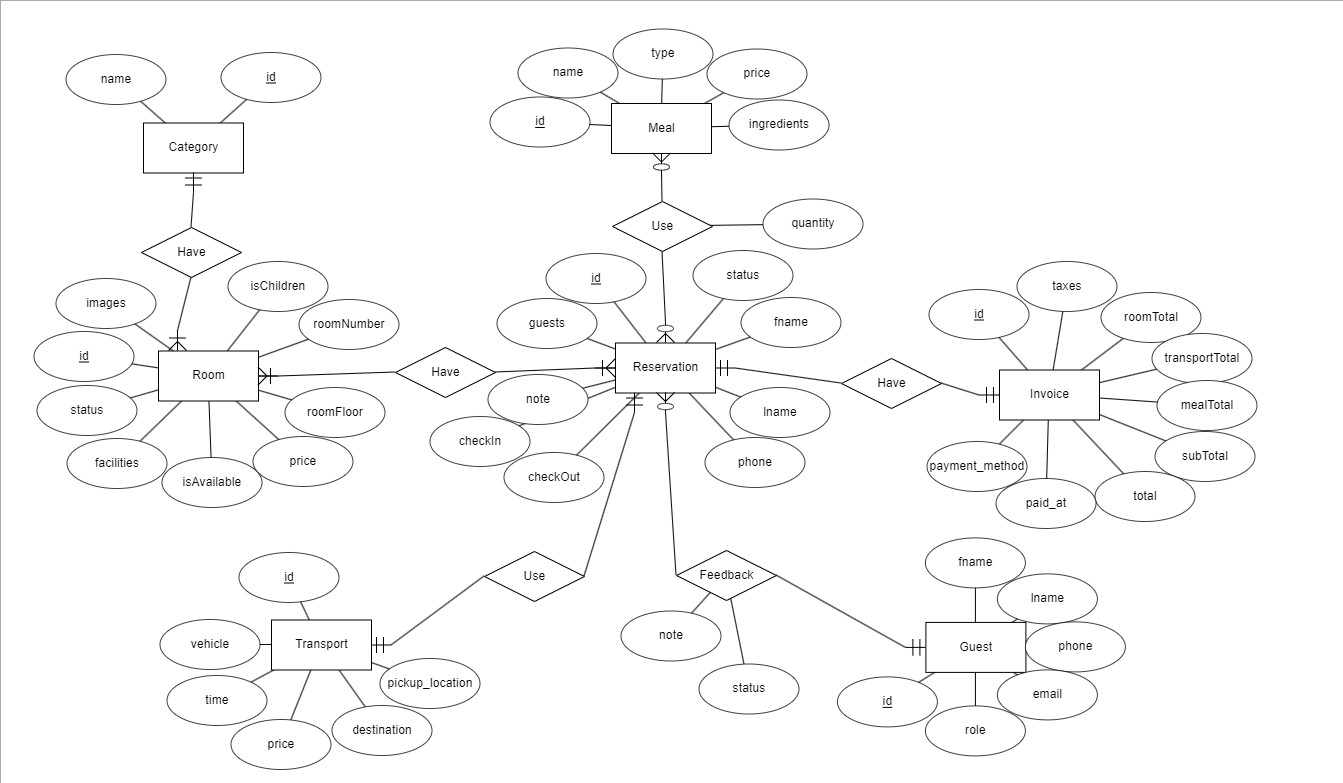
\includegraphics[width=\textwidth]{img/erd.jpg}
        \caption{Entity Relationship Diagram }
        \label{fig: Entity Relationship Diagram }
    \end{figure}
\section{Physical Database Design}
\begin{figure}[H]
    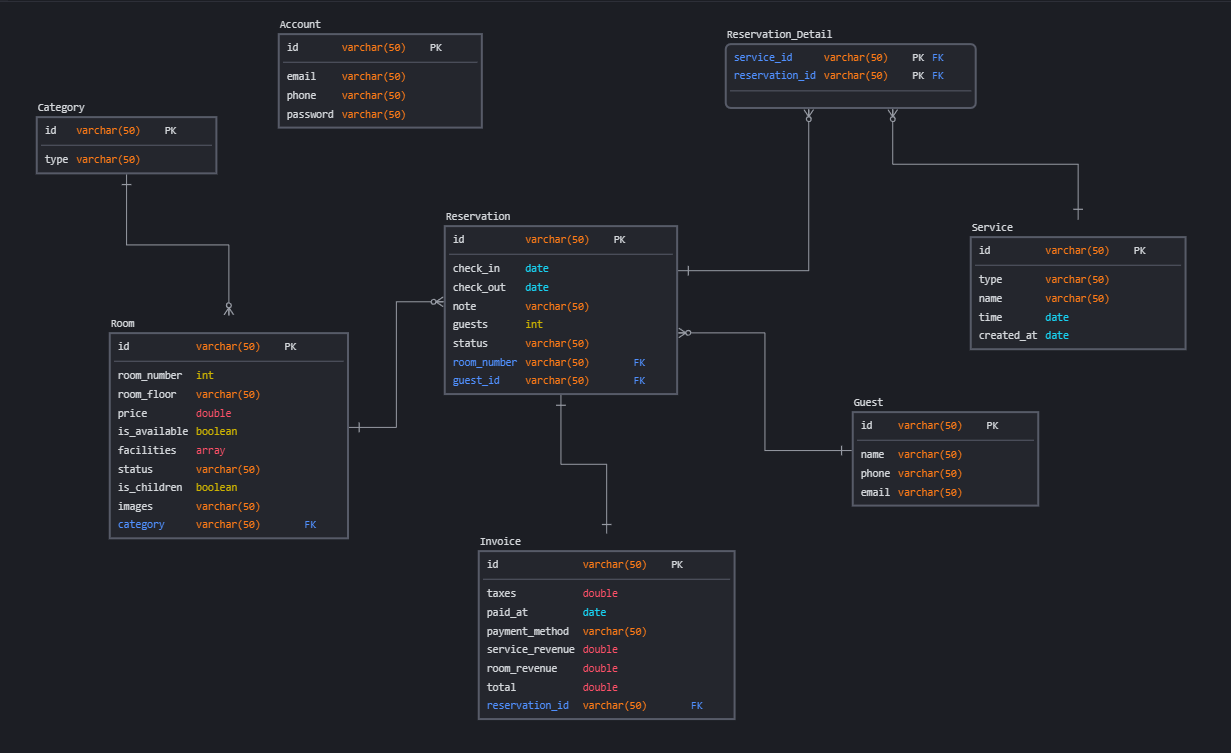
\includegraphics[width=1\linewidth]{img/physical_dtb.png}
    \caption{Physical Database Design}
    \label{fig:Physical Database Design}
\end{figure}
\section{Return on Investment(ROI)}
\begin{figure}[H]
        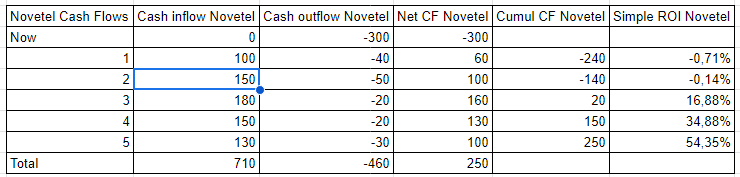
\includegraphics[width=\textwidth]{img/ROI.png}
        \caption{Return on Investment }
        \label{fig: ROI }
    \end{figure}

